\documentclass[tikz,border=16pt]{standalone}
\usepackage{amsmath,amssymb}
\usepackage{tikz}
\usetikzlibrary{arrows.meta, positioning, calc, fit, backgrounds, shapes.geometric}

%% ---- palette ----
\definecolor{cBlue}{RGB}{13,110,200}
\definecolor{cFillBlue}{RGB}{230,242,255}
\definecolor{cGray}{RGB}{95,108,120}
\definecolor{cFillGray}{RGB}{220,222,226}
\definecolor{cOrange}{RGB}{195,95,15}
\definecolor{cFillOrange}{RGB}{255,239,218}
\definecolor{cRed}{RGB}{170,35,35}
\definecolor{cFillRed}{RGB}{255,220,220}
\definecolor{cGreen}{RGB}{30,145,75}
\definecolor{cFillGreen}{RGB}{210,245,225}
\definecolor{cPurple}{RGB}{110,40,180}
\definecolor{cFillPurple}{RGB}{240,228,255}
\definecolor{cTeal}{RGB}{10,130,140}
\definecolor{cFillTeal}{RGB}{215,245,248}
\definecolor{cLegend}{RGB}{250,251,253}

\tikzset{
  actor/.style={rectangle, rounded corners=5pt, draw, minimum width=3.4cm,
                minimum height=0.8cm, font=\bfseries\small, align=center,
                inner sep=5pt, line width=1.4pt},
  actorVV/.style={actor, draw=cPurple, fill=cFillPurple, text=cPurple},
  actorSrc/.style={actor, draw=cBlue,  fill=cFillBlue,  text=cBlue},
  cbox/.style={rectangle, rounded corners=4pt, draw, minimum width=3.2cm,
               font=\scriptsize, align=left, inner sep=5pt, line width=1.1pt},
  cboxVV/.style={cbox, draw=cPurple, fill=cFillPurple, text=cPurple},
  cboxG/.style={cbox, draw=cGreen,  fill=cFillGreen,  text=cGreen},
  cboxR/.style={cbox, draw=cRed,    fill=cFillRed,    text=cRed},
  cboxO/.style={cbox, draw=cOrange, fill=cFillOrange, text=cOrange},
  cboxB/.style={cbox, draw=cBlue,   fill=cFillBlue,   text=cBlue},
  stepbubble/.style={circle, draw=cGray, fill=cFillGray, text=cGray,
                     font=\bfseries\scriptsize, inner sep=2pt, minimum size=0.5cm},
  msgarrow/.style={-{Stealth[length=7pt]}, line width=1.4pt},
  msgarrowB/.style={msgarrow, draw=cBlue},
  lifeline/.style={draw=cGray!40, line width=1pt, dashed},
  guard/.style={diamond, shape aspect=2.4, draw=cGray, fill=cFillGray, text=cGray,
                font=\bfseries\scriptsize, inner sep=2pt, align=center},
  guardR/.style={diamond, shape aspect=2.4, draw=cRed, fill=cFillRed, text=cRed,
                font=\bfseries\scriptsize, inner sep=2pt, align=center},
  guardG/.style={diamond, shape aspect=2.4, draw=cGreen, fill=cFillGreen, text=cGreen,
                font=\bfseries\scriptsize, inner sep=2pt, align=center},
}

\begin{document}
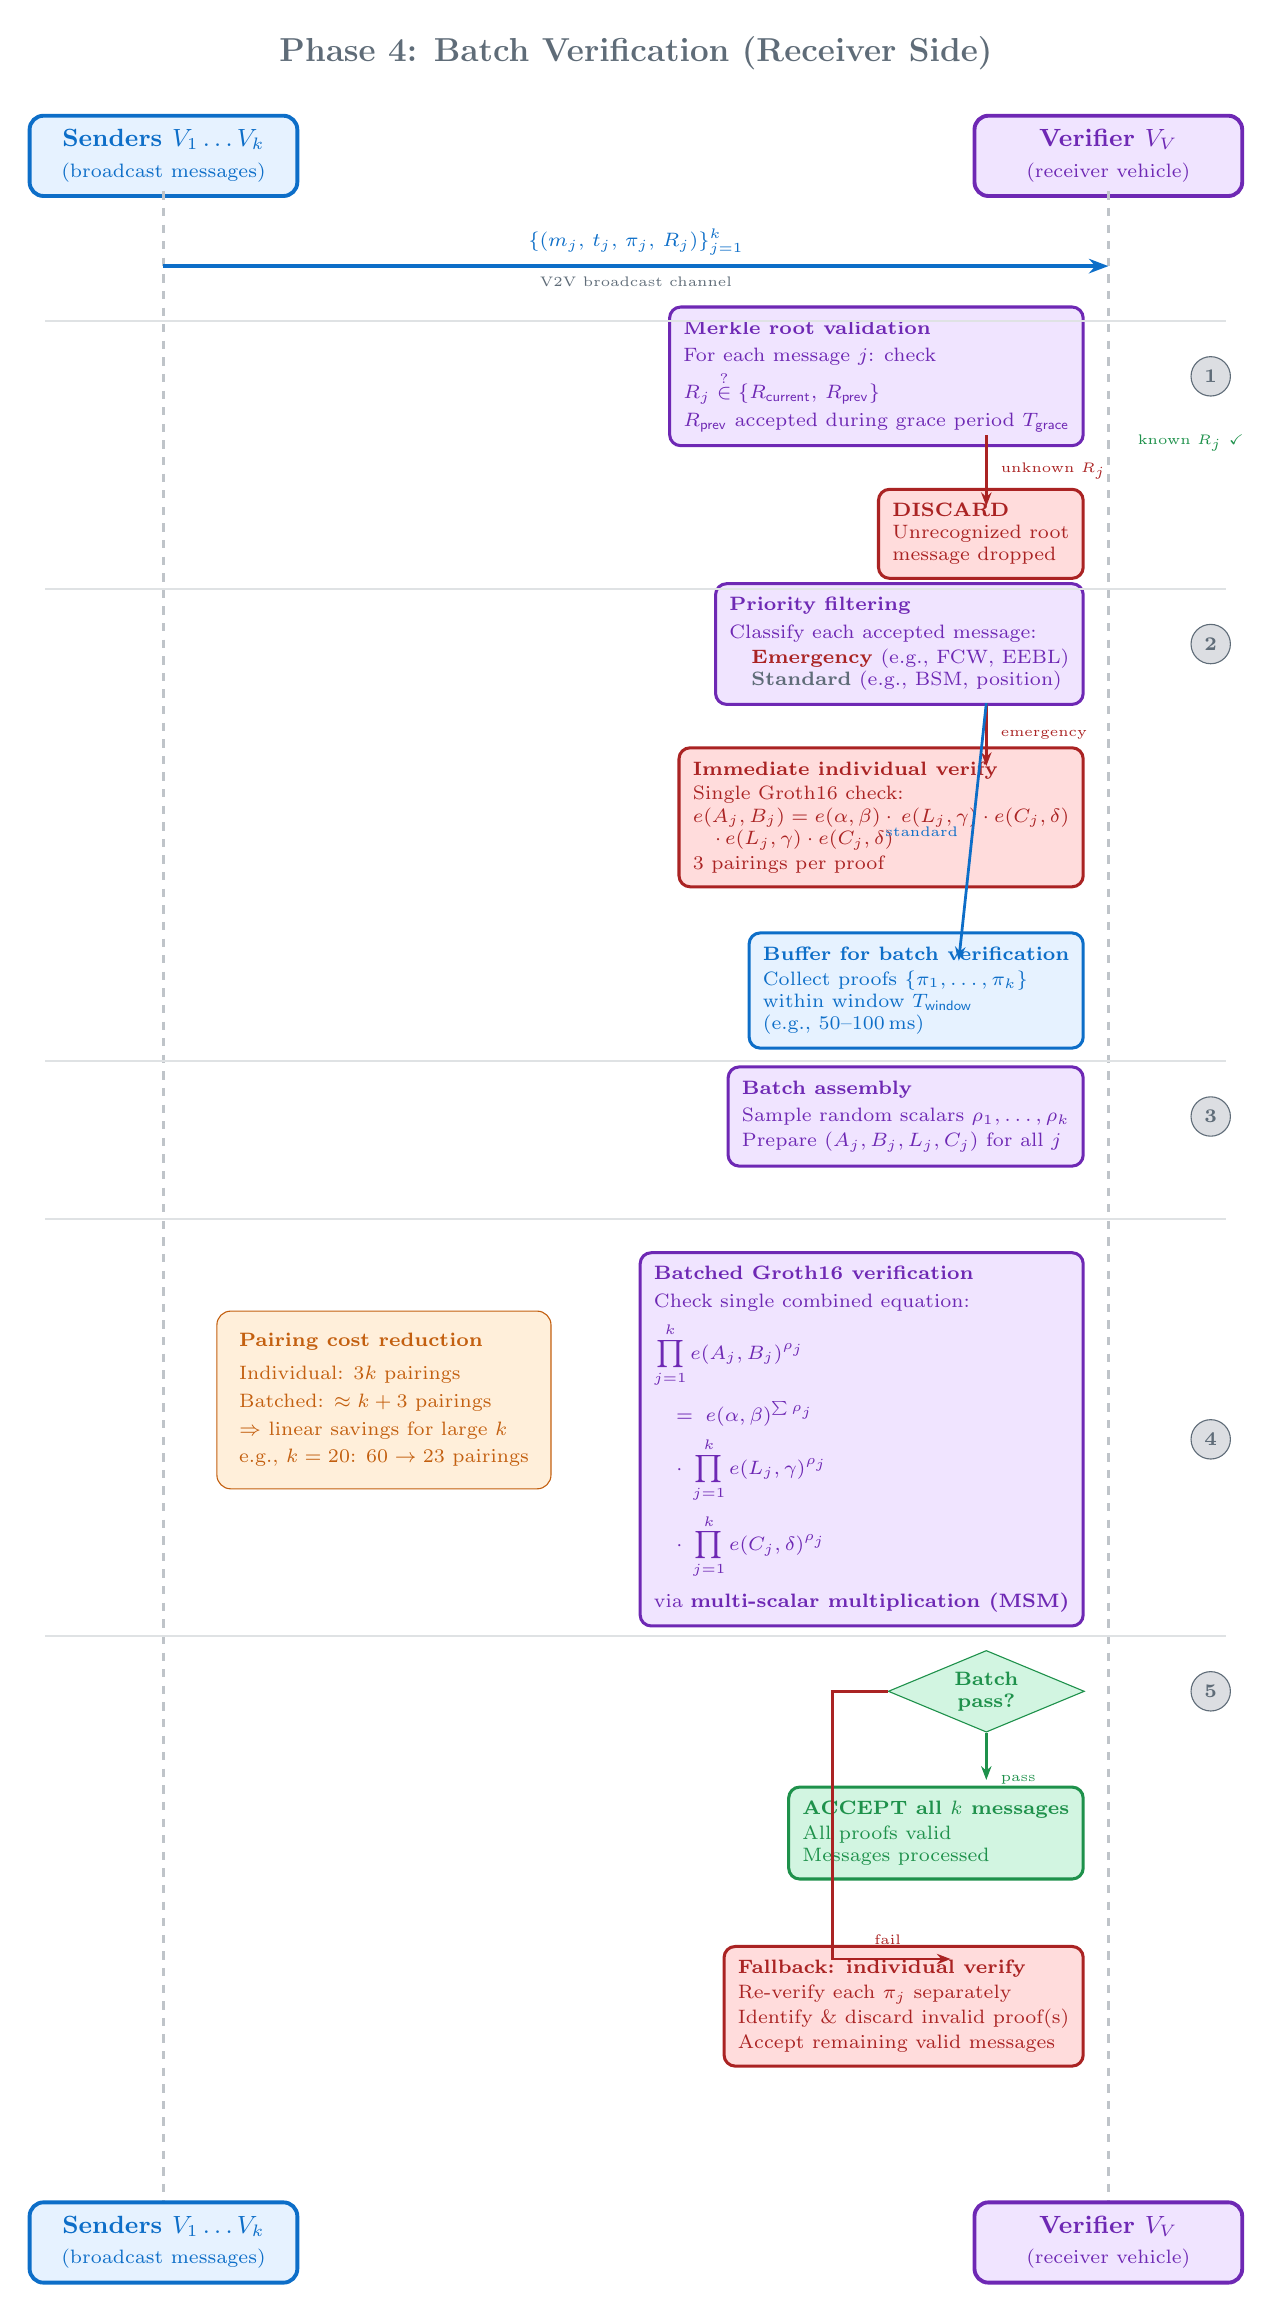
\begin{tikzpicture}

%% ============================================================
%%  ACTOR POSITIONS
%%  Sources (multiple Vi) at x=0,  Verifier VV at x=12
%% ============================================================
\def\Sx{0}
\def\VVx{12}

%% ----- Actor headers -----
\node[actorSrc] (Src) at (\Sx,  0) {Senders $V_1 \ldots V_k$\\{\scriptsize\normalfont (broadcast messages)}};
\node[actorVV]  (VV)  at (\VVx, 0) {Verifier $V_V$\\{\scriptsize\normalfont (receiver vehicle)}};

%% ----- Lifelines -----
\draw[lifeline] (\Sx,  -0.45) -- (\Sx,  -26.5);
\draw[lifeline] (\VVx, -0.45) -- (\VVx, -26.5);

%% ============================================================
%%  Incoming messages arrow  (y = -1.4)
%% ============================================================
\draw[msgarrowB] (\Sx, -1.4) -- (\VVx, -1.4)
  node[midway, above, font=\scriptsize\bfseries, text=cBlue]
    {$\{(m_j,\, t_j,\, \pi_j,\, R_j)\}_{j=1}^{k}$}
  node[midway, below, font=\tiny, text=cGray]
    {V2V broadcast channel};

%% ============================================================
%%  STEP 1 — Root check  (y = -2.8)
%% ============================================================
\def\ya{-2.8}
\node[stepbubble] at (\VVx+1.3, \ya) {1};
\node[cboxVV, anchor=east] at (\VVx-0.3, \ya) {%
  \textbf{Merkle root validation}\\[2pt]
  For each message $j$: check\\[1pt]
  $R_j \stackrel{?}{\in} \{R_{\mathsf{current}},\, R_{\mathsf{prev}}\}$\\[2pt]
  $R_{\mathsf{prev}}$ accepted during grace period $T_{\mathsf{grace}}$
};

%% discard branch
\node[cboxR, anchor=east, minimum width=2.6cm]
  at (\VVx-0.3, -4.8)
  {\textbf{DISCARD}\\Unrecognized root\\message dropped};
\draw[-{Stealth[length=5pt]}, cRed, line width=1pt]
  (\VVx-1.55, -3.55) -- (\VVx-1.55, -4.45)
  node[right, font=\tiny, text=cRed, midway, xshift=0.05cm] {unknown $R_j$};

%% pass annotation
\node[font=\tiny, text=cGreen] at (\VVx+1.05, -3.65) {known $R_j$ \checkmark};

%% ============================================================
%%  STEP 2 — Priority filter  (y = -6.2)
%% ============================================================
\def\yb{-6.2}
\node[stepbubble] at (\VVx+1.3, \yb) {2};
\node[cboxVV, anchor=east] at (\VVx-0.3, \yb) {%
  \textbf{Priority filtering}\\[2pt]
  Classify each accepted message:\\[1pt]
  \quad \textcolor{cRed}{\textbf{Emergency}} (e.g., FCW, EEBL)\\
  \quad \textcolor{cGray}{\textbf{Standard}} (e.g., BSM, position)
};

%% emergency branch — immediate verify
\node[cboxR, anchor=east, minimum width=3.2cm,
      draw=cRed, fill=cFillRed, text=cRed]
  at (\VVx-0.3, -8.4) {%
    \textbf{Immediate individual verify}\\[1pt]
    Single Groth16 check:\\
    $e(A_j,B_j) = e(\alpha,\beta)\cdot\, e(L_j,\gamma)\cdot e(C_j,\delta)$\\
    $\quad\cdot\, e(L_j,\gamma)\cdot e(C_j,\delta)$\\[1pt]
    3 pairings per proof
  };
\draw[-{Stealth[length=5pt]}, cRed, line width=1pt]
  (\VVx-1.55, -6.95) -- (\VVx-1.55, -7.75)
  node[right, font=\tiny, text=cRed, midway, xshift=0.05cm] {emergency};

%% standard branch — buffer
\node[cboxB, anchor=east, minimum width=3.2cm]
  at (\VVx-0.3, -10.6) {%
    \textbf{Buffer for batch verification}\\[1pt]
    Collect proofs $\{\pi_1,\ldots,\pi_k\}$\\
    within window $T_{\mathsf{window}}$\\
    (e.g., $50$--$100\,\mathrm{ms}$)
  };
\draw[-{Stealth[length=5pt]}, cBlue, line width=1pt]
  (\VVx-1.55, -6.95) -- (\VVx-0.3-3.2/2, -10.22)
  node[left, font=\tiny, text=cBlue, midway, xshift=-0.05cm] {standard};

%% ============================================================
%%  STEP 3 — Collect k proofs  (y = -12.2)
%% ============================================================
\def\yc{-12.2}
\node[stepbubble] at (\VVx+1.3, \yc) {3};
\node[cboxVV, anchor=east] at (\VVx-0.3, \yc) {%
  \textbf{Batch assembly}\\[2pt]
  Sample random scalars $\rho_1,\ldots,\rho_k$\\[1pt]
  Prepare $(A_j, B_j, L_j, C_j)$ for all $j$
};

%% ============================================================
%%  STEP 4 — Batched Groth16  (y = -14.3)
%% ============================================================
\def\yd{-16.3}
\node[stepbubble] at (\VVx+1.3, \yd) {4};
\node[cboxVV, anchor=east] at (\VVx-0.3, \yd) {%
  \textbf{Batched Groth16 verification}\\[2pt]
  Check single combined equation:\\[3pt]
  $\displaystyle\prod_{j=1}^{k} e(A_j,B_j)^{\rho_j}$\\[4pt]
  $\displaystyle\quad =\; e(\alpha,\beta)^{\sum\rho_j}$\\[3pt]
  $\displaystyle\quad\cdot\;\prod_{j=1}^{k} e(L_j,\gamma)^{\rho_j}$\\[3pt]
  $\displaystyle\quad\cdot\;\prod_{j=1}^{k} e(C_j,\delta)^{\rho_j}$\\[4pt]
  via \textbf{multi-scalar multiplication (MSM)}
};

%% pairing cost callout
\node[draw=cOrange, fill=cFillOrange, rounded corners=5pt,
      font=\scriptsize, align=left, inner sep=8pt, text=cOrange]
  at (2.8, -15.8) {%
    \textbf{Pairing cost reduction}\\[4pt]
    Individual: $3k$ pairings\\[2pt]
    Batched: $\approx k + 3$ pairings\\[2pt]
    $\Rightarrow$ linear savings for large $k$\\[2pt]
    e.g., $k=20$: $60 \to 23$ pairings
  };

%% ============================================================
%%  STEP 5 — Batch result guard  (y = -19.5)
%% ============================================================
\def\ye{-19.5}
\node[stepbubble] at (\VVx+1.3, \ye) {5};

\node[guardG, minimum width=2.2cm, minimum height=0.7cm]
  (guardBatch) at (\VVx-1.55, \ye) {Batch\\pass?};

%% pass
\node[cboxG, anchor=east, minimum width=2.8cm]
  at (\VVx-0.3, -21.3) {%
    \textbf{ACCEPT all $k$ messages}\\[1pt]
    All proofs valid\\
    Messages processed
  };
\draw[-{Stealth[length=5pt]}, cGreen, line width=1pt]
  (guardBatch.south) -- ++(0,-0.6)
  node[right, font=\tiny, text=cGreen, xshift=0.05cm] {pass};

%% fail — fallback
\node[cboxR, anchor=east, minimum width=3.2cm]
  at (\VVx-0.3, -23.5) {%
    \textbf{Fallback: individual verify}\\[1pt]
    Re-verify each $\pi_j$ separately\\[1pt]
    Identify \& discard invalid proof(s)\\[1pt]
    Accept remaining valid messages
  };
\draw[-{Stealth[length=5pt]}, cRed, line width=1pt]
  (guardBatch.west) -- ++(-0.7,0) -- ++(0,-3.4) -- ++(1.5, 0)
  node[above, font=\tiny, text=cRed, xshift=-0.8cm, yshift=0.05cm] {fail};

%% ============================================================
%%  TITLE
%% ============================================================
\node[font=\bfseries\large, text=cGray] at (6, 1.3)
  {Phase 4: Batch Verification (Receiver Side)};

%% ============================================================
%%  Horizontal separators
%% ============================================================
\foreach \yy in {-2.1, -5.5, -11.5, -13.5, -18.8} {
  \draw[cGray!20, line width=0.7pt] (-1.5, \yy) -- (13.5, \yy);
}

%% ============================================================
%%  Actor footers
%% ============================================================
\node[actorSrc] at (\Sx,  -26.5) {Senders $V_1 \ldots V_k$\\{\scriptsize\normalfont (broadcast messages)}};
\node[actorVV]  at (\VVx, -26.5) {Verifier $V_V$\\{\scriptsize\normalfont (receiver vehicle)}};

\end{tikzpicture}
\end{document}